% !TEX program = xelatex
\documentclass[notheorems,aspectratio=169]{beamer}
\usepackage{ctex,fontspec,xeCJK}
\IfFontExistsTF{Noto Serif CJK JP}{\setCJKmainfont{Noto Serif CJK JP}\setCJKsansfont{Noto Sans CJK JP}}{}
\usepackage{amsmath,amssymb,bm,booktabs,array,multicol}
\usepackage{tikz}
\usetikzlibrary{arrows.meta,calc,positioning,shapes.geometric,decorations.pathmorphing}
\usetheme{Madrid}
\usefonttheme[onlymath]{serif}
\beamertemplatenavigationsymbolsempty
\let\Tiny\tiny

\definecolor{ChinaRed}{RGB}{196,30,58}
\definecolor{JapanBlue}{RGB}{0,82,155}
\definecolor{SoftBlue}{RGB}{231,241,249}
\definecolor{SoftRed}{RGB}{252,235,239}
\definecolor{GraphGray}{RGB}{94,103,112}
\definecolor{ChemGreen}{RGB}{29,132,96}
\definecolor{SoftGreen}{RGB}{232,246,240}
\definecolor{Gold}{RGB}{215,153,33}
\setbeamercolor{structure}{fg=JapanBlue}
\setbeamercolor{alerted text}{fg=ChinaRed}
\setbeamercolor{block title alerted}{bg=ChinaRed,fg=white}
\setbeamercolor{block body alerted}{bg=SoftRed}
\setbeamercolor{block title}{bg=JapanBlue,fg=white}
\setbeamercolor{block body}{bg=SoftBlue}
\setbeamercolor{block title example}{bg=ChemGreen,fg=white}
\setbeamercolor{block body example}{bg=SoftGreen}
\setbeamertemplate{itemize item}{\color{JapanBlue}$\blacktriangleright$}
\setbeamertemplate{itemize subitem}{\color{ChinaRed}$\bullet$}
\newcommand{\jp}[1]{\textbf{\color{JapanBlue}#1}}
\newcommand{\key}[1]{\textbf{\color{ChinaRed}#1}}
\newcommand{\en}[1]{\textcolor{GraphGray}{\scriptsize(#1)}}
\newcommand{\ans}[1]{\textcolor{ChemGreen}{\textbf{答：}#1}}
\newcommand{\particle}[3]{\fill[#3] (#1,#2) circle (2.2pt);}
\setbeamercolor{question card}{fg=black,bg=SoftRed}
\setbeamercolor{answer card}{fg=black,bg=SoftGreen}
\newcommand{\questioncard}[1]{%
  \begin{columns}[c,onlytextwidth]
    \column{.10\textwidth}\centering
\begin{tikzpicture}\node[circle,fill=ChinaRed,text=white,font=\Large\bfseries,minimum size=10mm]{Q};\end{tikzpicture}
    \column{.87\textwidth}\begin{beamercolorbox}[rounded=true,shadow=true,sep=1.1ex]{question card}#1\end{beamercolorbox}
  \end{columns}}
\newcommand{\answercard}[1]{%
  \begin{columns}[c,onlytextwidth]
    \column{.10\textwidth}\centering
\begin{tikzpicture}\node[circle,fill=ChemGreen,text=white,font=\Large\bfseries,minimum size=10mm]{A};\end{tikzpicture}
    \column{.87\textwidth}\begin{beamercolorbox}[rounded=true,shadow=true,sep=1.1ex]{answer card}#1\end{beamercolorbox}
  \end{columns}}
\newcommand{\reasonflow}[3]{%
  \begin{center}\begin{tikzpicture}[>=Latex,node distance=5mm,flow/.style={draw=JapanBlue,fill=SoftBlue,rounded corners=2mm,minimum width=30mm,minimum height=9mm,align=center,font=\small\bfseries}]
    \node[flow] (a) {#1};\node[flow,right=of a] (b) {#2};\node[flow,right=of b] (c) {#3};
    \draw[->,very thick,ChinaRed] (a)--(b);\draw[->,very thick,ChinaRed] (b)--(c);
  \end{tikzpicture}\end{center}}
\title[EJU Chemistry]{化学1}
\subtitle{物質の分類・分離と精製・元素・三態・原子と同位体}
\author[Sirui Liu]{Sirui Liu}
\date{2026年7月}

\begin{document}
\begin{frame}\titlepage\end{frame}
\begin{frame}{目次}\tableofcontents\end{frame}

\section{物質の分類}
\begin{frame}{物質の分類：全体像}
\centering
\begin{tikzpicture}[node distance=5mm and 9mm,box/.style={draw,rounded corners,minimum width=28mm,minimum height=8mm,align=center,font=\small},>=Latex]
\node[box,fill=SoftBlue,draw=JapanBlue] (m) {物質};
\node[box,fill=SoftBlue,draw=JapanBlue,below left=of m] (p) {純物質\en{pure substance}};
\node[box,fill=SoftRed,draw=ChinaRed,below right=of m] (x) {混合物\en{mixture}};
\node[box,fill=SoftGreen,draw=ChemGreen,below left=of p] (s) {単体\en{simple substance}};
\node[box,fill=SoftGreen,draw=ChemGreen,below right=of p] (c) {化合物\en{compound}};
\draw[->,thick] (m)--(p);\draw[->,thick] (m)--(x);\draw[->,thick] (p)--(s);\draw[->,thick] (p)--(c);
\node[below=2mm of s,font=\scriptsize] {Fe, O$_2$, S$_8$};
\node[below=2mm of c,font=\scriptsize] {H$_2$O, NaCl, CO$_2$};
\node[below=2mm of x,font=\scriptsize] {空気、海水、原油};
\end{tikzpicture}
\begin{alertblock}{判断顺序}先判断组成是否固定，再判断能否用化学变化分解。\end{alertblock}
\end{frame}

\begin{frame}{純物質（纯物质）と混合物（混合物）}
\begin{columns}[T,onlytextwidth]
\column{.48\textwidth}\begin{block}{純物質}\begin{itemize}\item 只含一种物质，组成固定\item 熔点・沸点通常固定\item 例：水、酸素、塩化ナトリウム\end{itemize}\end{block}
\column{.48\textwidth}\begin{alertblock}{混合物}\begin{itemize}\item 两种以上物质混合，比例可变\item 熔点・沸点常为范围\item 例：空気、海水、石油\end{itemize}\end{alertblock}
\end{columns}
\begin{exampleblock}{ミニ例題}食塩水、酸素、空気、水を分類せよ。\quad \ans{純物質：酸素・水；混合物：食塩水・空気。}\end{exampleblock}
\end{frame}

\begin{frame}{図例：粒子から見分ける}
\centering
\begin{tikzpicture}[font=\small]
\draw[rounded corners,very thick,JapanBlue,fill=SoftBlue] (-5,-1.7) rectangle (-.5,1.7);
\draw[rounded corners,very thick,ChinaRed,fill=SoftRed] (.5,-1.7) rectangle (5,1.7);
\foreach \x/\y in {-4.3/1,-3.2/.9,-2.1/1.15,-1.1/.8,-4/.1,-2.8/0,-1.6/.2,-4.2/-.9,-3/-.8,-1.7/-1}{\particle{\x}{\y}{JapanBlue}}
\foreach \x/\y in {1.2/1,2.8/.9,4.2/1.1,1.5/0,3.3/.1,4.5/-.1,1.1/-1,2.6/-.8,4/-1}{\particle{\x}{\y}{ChinaRed}}
\foreach \x/\y in {2/.7,3.7/.55,2.2/-.25,3.2/-1.15}{\particle{\x}{\y}{ChemGreen}}
\node[font=\bfseries] at (-2.75,2.05) {純物質：同一种粒子};
\node[font=\bfseries] at (2.75,2.05) {混合物：两种以上粒子};
\node[align=center] at (-2.75,-2.15) {例：酸素 O$_2$};
\node[align=center] at (2.75,-2.15) {例：空気（N$_2$, O$_2$, Ar, \dots）};
\end{tikzpicture}
\begin{exampleblock}{EJU形式}同一种分子だけが描かれた粒子図はどちらか。\quad \ans{左。粒子种类只有一种。}\end{exampleblock}
\end{frame}

\begin{frame}{単体・化合物・元素}
\small
\begin{tabular}{p{18mm}p{61mm}p{27mm}}\toprule
用語 & 意味 & 例\\\midrule
単体（单质）& 一种元素构成的純物質 & O$_2$, O$_3$, Fe\\
化合物（化合物）& 两种以上元素按固定比例结合的純物質 & H$_2$O, CO$_2$\\
元素（元素）& 具有相同原子番号的一类原子的总称 & O, C, Fe\\\bottomrule\end{tabular}
\begin{exampleblock}{EJU形式}O$_2$ と O$_3$ は構造と性質が異なるが、同じ酸素元素からなる。この関係を何というか。\quad \ans{同素体。}\end{exampleblock}
\end{frame}

\section{混合物の分離と精製}
\begin{frame}{分離と精製：利用する性質}
\small\centering
\begin{tabular}{lll}\toprule 性質の差 & 方法 & 典型例\\\midrule
粒子大小・不溶性 & ろ過 & 砂と水\\
沸点 & 蒸留・分留 & 食塩水、原油\\
溶解度の温度変化 & 再結晶 & 硝酸カリウム\\
溶媒への溶けやすさ & 抽出 & ヨウ素水\\
吸着・移動速度 & クロマトグラフィー & インク\\
昇華性 & 昇華法 & ヨウ素と砂\\\bottomrule\end{tabular}
\begin{exampleblock}{方法選択}海水から純水を回収し、残った塩も得たい。操作の順序は？\quad \ans{先蒸留回收水，再从残液蒸发・結晶化得到塩。}\end{exampleblock}
\end{frame}

\begin{frame}{ろ過：不溶性固体を分ける}
\begin{columns}[c,onlytextwidth]\column{.44\textwidth}
\centering\begin{tikzpicture}[scale=.85]
\draw[thick] (-1.4,2.4)--(0,0)--(1.4,2.4);\draw[thick,JapanBlue] (-1.05,2.15)--(0,.35)--(1.05,2.15);
\fill[GraphGray!55] (-.72,1.65)--(0,.48)--(.72,1.65)--cycle;
\draw[thick] (-.8,-.25)--(-.58,-2.25)--(.58,-2.25)--(.8,-.25);\fill[SoftBlue] (-.62,-1.3) rectangle (.62,-2.18);
\draw[->,ChinaRed,very thick] (0,.25)--(0,-.8);\node[right] at (1.05,1.8){ろ紙};\node[right] at (.65,-1.75){ろ液};
\end{tikzpicture}
\column{.52\textwidth}\begin{block}{操作要点}\begin{itemize}\item 液体沿玻璃棒流下\item ろ紙边缘低于漏斗边缘\item 漏斗脚尖贴住烧杯内壁\end{itemize}\end{block}\end{columns}
\end{frame}

\begin{frame}{ろ過：例題}
\def\exq{砂、食塩、水の混合物をろ過した。ろ液を蒸発皿で乾固すると白色固体が残った。この固体は何か。また、なぜろ液に入ったか。}
\only<1>{\vfill\questioncard{\exq}\vfill}
\only<2>{\questioncard{\exq}\vfill\reasonflow{食塩は水に溶ける}{溶質はろ紙を通る}{乾固で結晶が残る}\vfill
\answercard{白色固体は\jp{塩化ナトリウム}。溶けた食塩は水とともにろ紙を通過し、ろ液に含まれた。}}
\end{frame}

\begin{frame}{蒸留：沸点差を利用}
\begin{columns}[c,onlytextwidth]\column{.56\textwidth}
\centering\begin{tikzpicture}[scale=.78,>=Latex]
\draw[thick] (-3,-.8) circle (.75);\fill[SoftBlue] (-3,-1.2) arc (225:315:1.05) -- cycle;
\draw[thick] (-3,.0)--(-3,1.0)--(-1.4,1.0);\draw[thick] (-1.4,.72) rectangle (1.5,1.28);\draw[thick] (1.5,1)--(2.4,-.2);
\draw[thick] (2,-.4)--(2.15,-1.6)--(3.2,-1.6)--(3.35,-.4);\fill[SoftBlue] (2.12,-1.1) rectangle (3.23,-1.55);
\draw[->,JapanBlue,thick] (1.1,.6)--(-.7,.6);\node[below,font=\scriptsize] at (.3,.55){冷却水：下から上};
\draw[decorate,decoration={snake,amplitude=1mm},ChinaRed,thick] (-3,-1.8)--(-3,-1.45);\node[below] at (-3,-1.85){加熱};
\end{tikzpicture}
\column{.4\textwidth}\begin{block}{过程}\begin{enumerate}\item 低沸点成分气化\item 蒸気进入冷却器\item 液化后回收\end{enumerate}\end{block}\end{columns}
\end{frame}

\begin{frame}{蒸留：例題}
\def\exq{食塩水の蒸留装置で、冷却水を冷却器の上端から入れていた。どこを直すべきか。また、受器に集まる主成分は何か。}
\only<1>{\vfill\questioncard{\exq}\vfill}
\only<2>{\questioncard{\exq}\vfill\reasonflow{冷却水は下端から}{套管を水で満たす}{水蒸気を十分冷却}\vfill
\answercard{冷却水を\key{下端から入れ、上端から出す}。受器の主成分は\jp{水}。塩化ナトリウムはフラスコに残る。}}
\end{frame}

\begin{frame}{分留：多个沸点段}
\begin{columns}[T,onlytextwidth]\column{.5\textwidth}
\begin{block}{分留（fractional distillation）}通过分馏塔反复进行气化与液化，将沸点接近的液体分成若干\jp{留分}。\end{block}
\column{.46\textwidth}
\centering\begin{tikzpicture}[scale=.8]\draw[thick] (0,0) rectangle (2.2,4);\foreach \y in {.6,1.2,1.8,2.4,3,3.6}{\draw (0,\y)--(2.2,\y);}\draw[->,ChinaRed,thick] (1.1,-.5)--(1.1,4.5);\node[right] at (2.3,3.5){低沸点};\node[right] at (2.3,.4){高沸点};\end{tikzpicture}
\end{columns}
\begin{exampleblock}{例題}原油に単純な蒸留ではなく分留塔を使う理由は？\quad \ans{多种液体的沸点较接近，需要反复气化・液化提高分离效果。}\end{exampleblock}
\end{frame}

\begin{frame}{再結晶：溶解度曲線で理解}
\begin{columns}[c,onlytextwidth]\column{.59\textwidth}
\centering\begin{tikzpicture}[x=.055cm,y=.024cm,>=Latex]
\draw[->] (0,0)--(105,0) node[right]{温度/\,$^\circ$C};\draw[->] (0,0)--(0,190) node[above,align=center]{溶解度\\g/100 g 水};
\draw[JapanBlue,very thick] plot[smooth] coordinates{(0,13)(20,32)(40,64)(60,110)(80,169)(100,190)};
\draw[ChinaRed,very thick] plot[smooth] coordinates{(0,35)(20,36)(40,37)(60,38)(80,39)(100,40)};
\node[JapanBlue] at (73,145){硝酸カリウム};\node[ChinaRed] at (76,48){塩化ナトリウム};
\draw[dashed] (20,0)--(20,32);\draw[dashed] (80,0)--(80,169);
\end{tikzpicture}
\column{.37\textwidth}\begin{block}{意味}\begin{itemize}\item 高温で溶かす\item 冷却すると溶解度が低下\item 余分な溶質が結晶として析出\end{itemize}\end{block}\end{columns}
\end{frame}

\begin{frame}{再結晶：例題}
\def\exq{水100 gの80\,$^\circ$C飽和溶液を20\,$^\circ$Cまで冷却する。溶解度を硝酸カリウム169→32、塩化ナトリウム39→36 g/100 g水とすると、各析出量は？}
\only<1>{\vfill\questioncard{\exq}\vfill}
\only<2>{\questioncard{\exq}\vfill\reasonflow{高温の溶解量}{低温でも溶ける量}{差が析出量}\vfill
\answercard{\centering $\mathrm{KNO_3}:169-32=\boxed{137\,g}$\qquad $\mathrm{NaCl}:39-36=\boxed{3\,g}$\quad 溶解度曲線が急な物質ほど多く析出する。}}
\end{frame}

\begin{frame}{抽出：溶媒への溶けやすさ}
\begin{columns}[c,onlytextwidth]\column{.45\textwidth}
\centering\begin{tikzpicture}[scale=.85]
\draw[thick] (-.8,2.8)--(.8,2.8)--(.48,1.9)--(.48,.5)--(.15,-1.2)--(-.15,-1.2)--(-.48,.5)--(-.48,1.9)--cycle;
\fill[SoftRed] (-.45,.55) rectangle (.45,1.55);\fill[SoftBlue] (-.45,-.05)--(-.15,-1.1)--(.15,-1.1)--(.45,-.05)--cycle;
\draw[thick] (0,-1.2)--(0,-1.65);\draw[thick] (-.45,-1.5)--(.45,-1.5);\node[right] at (.6,1.05){有機層};\node[right] at (.6,-.45){水層};
\end{tikzpicture}
\column{.51\textwidth}\begin{block}{抽出（extraction）}\begin{enumerate}\item 混ざり合わない溶媒を加える\item 振って溶質を移す\item 静置して二層を分ける\end{enumerate}\end{block}\end{columns}
\begin{alertblock}{要点}上下由\key{密度}决定；目标物进入哪一层由\key{溶解度}决定。\end{alertblock}
\end{frame}

\begin{frame}{抽出：例題}
\def\exq{ヨウ素水にヘキサン（密度0.66 g/cm$^3$）を加えて振った。静置後、上層・下層のどちらが紫色になるか。理由も答えよ。}
\only<1>{\vfill\questioncard{\exq}\vfill}
\only<2>{\questioncard{\exq}\vfill\reasonflow{密度が水より小さい}{ヘキサンは上層}{ヨウ素がよく溶ける}\vfill
\answercard{\jp{上層}が紫色。ヘキサンは水より密度が小さく上層となり、ヨウ素は水よりヘキサンに溶けやすい。}}
\end{frame}

\begin{frame}{クロマトグラフィー：移動速度の差}
\centering\begin{tikzpicture}[scale=.9]
\draw[thick] (-4,-1.3) rectangle (-1,2);\draw[JapanBlue,thick] (-4,-.9)--(-1,-.9);\fill[SoftBlue] (-4,-1.3) rectangle (-1,-.9);
\fill[ChinaRed] (-2.5,-.65) circle (3pt);\draw[->,very thick] (-.3,.3)--(.8,.3);
\draw[thick] (1.2,-1.3) rectangle (4.2,2);\draw[JapanBlue,thick] (1.2,1.55)--(4.2,1.55);\fill[ChinaRed] (2.7,1.0) circle (3pt);\fill[ChemGreen] (2.7,.15) circle (3pt);\fill[Gold] (2.7,-.55) circle (3pt);
\node at (-2.5,2.35){展開前};\node at (2.7,2.35){展開後};
\end{tikzpicture}
\begin{block}{原理}固定相への吸着の強さ、移動相への溶けやすさの差で移動距離が変わる。\end{block}
\end{frame}

\begin{frame}{クロマトグラフィー：例題}
\def\exq{溶媒前線が8.0 cm、赤色色素が6.0 cm、青色色素が2.4 cm移動した。各$R_f$値と、紙により強く吸着した色素を答えよ。}
\only<1>{\vfill\questioncard{\exq}\vfill}
\only<2>{\questioncard{\exq}\vfill\reasonflow{$R_f=\text{色素}/\text{前線}$}{赤0.75・青0.30}{小さい方が強く吸着}\vfill
\answercard{$R_f(赤)=6.0/8.0=\jp{0.75}$、$R_f(青)=2.4/8.0=\jp{0.30}$。紙により強く吸着したのは\key{青色色素}。}}
\end{frame}

\begin{frame}{昇華法：固体から直接気体へ}
\begin{columns}[c,onlytextwidth]\column{.48\textwidth}
\centering\begin{tikzpicture}[scale=.9]
\fill[GraphGray!30] (-1.6,-1.3) rectangle (1.6,-.8);\draw[thick] (-1.8,-1.3)--(-1.5,1.3)--(1.5,1.3)--(1.8,-1.3)--cycle;
\draw[thick] (-1.5,1.3)--(0,2.3)--(1.5,1.3);\foreach \x in {-1,-.5,0,.5,1}{\draw[->,ChinaRed] (\x,-.7)--(\x,1.0);}\foreach \x in {-1,-.55,0,.55,1}{\fill[JapanBlue] (\x,1.45) circle (2pt);}
\node at (0,-1.75){ヨウ素＋砂};\node at (0,2.65){冷面上析出ヨウ素};
\end{tikzpicture}
\column{.48\textwidth}\begin{block}{昇華（sublimation）}\[\text{固体}\rightleftarrows\text{気体}\]液体阶段を経ない。ヨウ素、ナフタレン、ドライアイスなど。\end{block}\end{columns}
\end{frame}

\begin{frame}{昇華法：例題}
\def\exq{ヨウ素と砂の混合物をビーカーで穏やかに加熱し、上を冷たい時計皿で覆った。結晶が付着する場所と、砂が残る理由を答えよ。}
\only<1>{\vfill\questioncard{\exq}\vfill}
\only<2>{\questioncard{\exq}\vfill\reasonflow{ヨウ素だけ昇華}{蒸気が上へ移動}{冷面で固体へ戻る}\vfill
\answercard{ヨウ素の結晶は\jp{時計皿の下面}に付着する。砂はこの温度で昇華しないため、ビーカー内に残る。}}
\end{frame}

\begin{frame}{分離法を選ぶ：総合例題}
\small\begin{tabular}{p{55mm}p{44mm}}\toprule 操作场景 & 方法\\\midrule
泥水から水を通過させる & ろ過\\
食塩水から水を回収する & 蒸留\\
原油を沸点範囲ごとに分ける & 分留\\
熱水溶液を冷やして結晶を得る & 再結晶\\
ヨウ素水からヨウ素を有機溶媒へ移す & 抽出\\
インクの色素を分ける & クロマトグラフィー\\
ヨウ素と砂を分ける & 昇華法\\\bottomrule\end{tabular}
\end{frame}

\section{元素・同素体・元素の確認}
\begin{frame}{元素と同素体}
\begin{block}{同素体（同素异形体）}同じ元素からなる単体で、構造と性質が異なるもの。\end{block}
\centering\begin{tabular}{ll}\toprule 元素 & 代表的な同素体\\\midrule
炭素 C & ダイヤモンド、黒鉛、フラーレン、カーボンナノチューブ\\
酸素 O & 酸素 O$_2$、オゾン O$_3$\\
リン P & 黄リン、赤リン\\
硫黄 S & 斜方硫黄、単斜硫黄、ゴム状硫黄\\\bottomrule\end{tabular}
\begin{exampleblock}{例題}O$_2$ と O$_3$ の関係は？\quad \ans{酸素元素的同素体。}\end{exampleblock}
\end{frame}

\begin{frame}{炭素の同素体 I：ダイヤモンド}
\begin{columns}[c,onlytextwidth]\column{.5\textwidth}
\centering\begin{tikzpicture}[scale=.85]
\coordinate (C) at (0,0);
\draw[very thick,GraphGray] (C)--(-1.55,.65);\draw[very thick,GraphGray] (C)--(1.55,.65);
\draw[very thick,dashed,GraphGray] (C)--(0,1.65);
\fill[GraphGray!75] (C)--(-.2,-.2)--(0,-1.75)--(.2,-.2)--cycle;
\foreach \x/\y in {-1.55/.65,1.55/.65,0/1.65,0/-1.75}{\fill[JapanBlue] (\x,\y) circle (4pt);\draw[GraphGray] (\x,\y)--++(.5,.45);\draw[GraphGray] (\x,\y)--++(-.5,.45);}
\fill[ChinaRed] (C) circle (5pt);
\node[below] at (0,-2.25){各Cが4個のCと共有結合};
\end{tikzpicture}
\column{.46\textwidth}\begin{itemize}\item 三维网状结构\item 非常硬、融点高\item 自由电子がなく、電気を通しにくい\end{itemize}\end{columns}
\begin{exampleblock}{例題}ダイヤモンドが硬い理由は？\quad \ans{强固的共有結合在三维方向连续。}\end{exampleblock}
\end{frame}

\begin{frame}{炭素の同素体 II：黒鉛}
\begin{columns}[c,onlytextwidth]\column{.57\textwidth}
\centering\begin{tikzpicture}[scale=.72]
\foreach \dy in {0,1.45}{\foreach \x in {-2.4,-.8,.8,2.4}{\draw[very thick,GraphGray] (\x,\dy) ++(0:0.75) \foreach \a in {60,120,180,240,300,360}{--++(\a:0.75)};}}
\foreach \x in {-2.4,-.8,.8,2.4}{\draw[dashed,ChinaRed] (\x,-.1)--(\x,1.35);}
\node at (0,-1){层间作用弱，可滑动};
\end{tikzpicture}
\column{.39\textwidth}\begin{itemize}\item 六角网状平面が層状に重なる\item 各Cは3個と結合\item 自由に動ける電子があり、導電性を示す\end{itemize}\end{columns}
\begin{exampleblock}{例題}黒鉛が鉛筆芯と電極に使える理由を一つずつ答えよ。\quad \ans{层易滑动；有导电性。}\end{exampleblock}
\end{frame}

\begin{frame}{炭素の同素体 III：フラーレンとナノチューブ}
\begin{columns}[c,onlytextwidth]\column{.48\textwidth}\centering
\begin{tikzpicture}[scale=.8]\draw[very thick,JapanBlue] (0,0) circle (1.7);\foreach \a in {0,36,...,324}{\draw[GraphGray] (0,0)--(\a:1.7);}\draw[ChinaRed,thick] (0,0) ++(90:.62) \foreach \a in {162,234,306,18,90}{--++(\a:.73)};\node at (0,-2.2){フラーレン C$_{60}$};\node[font=\scriptsize] at (0,-2.65){五角形＋六角形の閉じたかご};\end{tikzpicture}
\column{.48\textwidth}\centering
\begin{tikzpicture}[scale=.8]\draw[very thick,JapanBlue] (-1.6,-1.6) arc (180:360:1.6 and .45);\draw[very thick,JapanBlue] (-1.6,1.6) arc (180:540:1.6 and .45);\draw[very thick,JapanBlue] (-1.6,-1.6)--(-1.6,1.6);\draw[very thick,JapanBlue] (1.6,-1.6)--(1.6,1.6);\foreach \x in {-1.2,-.4,.4,1.2}{\draw[GraphGray] (\x,-1.5)--(\x,1.5);}\foreach \y in {-1,-.3,.4,1.1}{\draw[GraphGray] (-1.55,\y) arc (180:360:1.55 and .42);}\node at (0,-2.2){カーボンナノチューブ};\node[font=\scriptsize] at (0,-2.65){黒鉛のシートを筒状にした構造};\end{tikzpicture}\end{columns}
\begin{exampleblock}{例題}二者に共通する元素は？\quad \ans{炭素。结构不同，所以性质不同。}\end{exampleblock}
\end{frame}

\begin{frame}{酸素の同素体：O$_2$ と O$_3$}
\begin{columns}[T,onlytextwidth]\column{.48\textwidth}\begin{block}{酸素 O$_2$}\begin{itemize}\item 无色无臭\item 助燃性\item 大气中约21\%\end{itemize}\end{block}
\column{.48\textwidth}\begin{alertblock}{オゾン O$_3$}\begin{itemize}\item 淡青色、有特有臭味\item 強い酸化力\item 紫外線吸収に重要\end{itemize}\end{alertblock}\end{columns}
\begin{exampleblock}{例題}漂白・殺菌に使われる酸素の同素体は？\quad \ans{オゾン O$_3$。}\end{exampleblock}
\end{frame}

\begin{frame}{リンの同素体：黄リンと赤リン}
\small\begin{tabular}{lll}\toprule & 黄リン & 赤リン\\\midrule 色 & 淡黄色 & 赤褐色\\ 毒性 & 強い & 黄リンより低い\\ 発火 & 空気中で自然発火しやすい & 比較的安定\\ 保存 & 水中 & 密閉容器\\\bottomrule\end{tabular}
\begin{exampleblock}{例題}黄リンを水中保存する主な理由は？\quad \ans{隔绝空气，防止自然発火。}\end{exampleblock}
\end{frame}

\begin{frame}{硫黄の同素体}
\small\centering\begin{tabular}{llll}\toprule & 斜方硫黄 & 単斜硫黄 & ゴム状硫黄\\\midrule 外形 & 八面体 & 針状 & 弹性状\\ 分子 & S$_8$ & S$_8$ & 长链状\\ 常温安定性 & 最稳定 & 斜方へ変化 & 徐々に硬化\\ 作り方 & CS$_2$から結晶 & 溶融硫黄を徐冷 & 溶融硫黄を冷水へ\\\bottomrule\end{tabular}
\begin{exampleblock}{例題}常温で最も安定な硫黄は？\quad \ans{斜方硫黄。}\end{exampleblock}
\end{frame}

\begin{frame}{炎色反応：元素の確認}
\centering\begin{tabular}{ccccccc}\toprule 元素 & Li & Na & K & Ca & Sr & Cu\\\midrule 色 & 赤 & 黄 & 紫 & 橙赤 & 紅 & 青緑\\\bottomrule\end{tabular}
\vspace{1em}
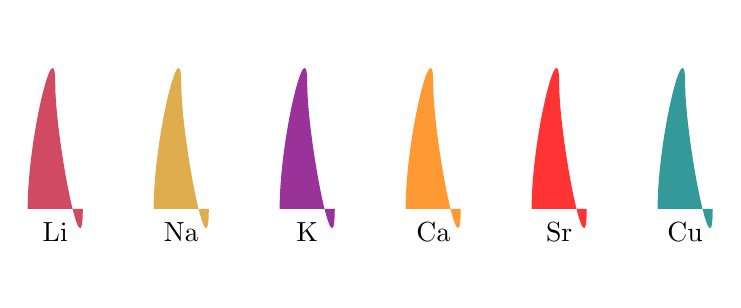
\begin{tikzpicture}\foreach \x/\c/\t in {0/ChinaRed/Li,1.6/Gold/Na,3.2/violet/K,4.8/orange/Ca,6.4/red/Sr,8/teal/Cu}{\fill[\c!80] (\x,0) .. controls +(0,.9) and +(0,.7) .. (\x+.35,1.6) .. controls +(0,-.7) and +(0,-.9) .. (\x+.7,0)--cycle;\node at (\x+.35,-.3){\t};}\end{tikzpicture}
\begin{exampleblock}{例題}炎色が黄色なら最も疑われる元素は？\quad \ans{ナトリウム Na。}\end{exampleblock}
\end{frame}

\begin{frame}{沈殿・気体による元素の確認}
\small\begin{tabular}{lll}\toprule 操作 & 观察 & 确认\\\midrule
塩化物イオン＋硝酸銀水溶液 & 白色沈殿 AgCl & 塩素 Cl\\
硫酸イオン＋塩化バリウム水溶液 & 白色沈殿 BaSO$_4$ & 硫黄 S\\
二酸化炭素＋石灰水 & 白く濁る CaCO$_3$ & 炭素 C\\
有機物を燃焼→水 & 塩化コバルト紙が赤色 & 水素 H\\\bottomrule\end{tabular}
\begin{exampleblock}{例題}未知物質を燃焼させ、生成気体を石灰水に通すと白濁した。含まれる元素は？\quad \ans{炭素。}\end{exampleblock}
\end{frame}

\section{熱運動と三態変化}
\begin{frame}{熱運動と拡散}
\begin{block}{熱運動（thermal motion）}粒子が不断进行的无规则运动。温度越高，平均动能越大，运动越剧烈。\end{block}
\centering\begin{tikzpicture}[>=Latex]\draw[rounded corners,thick] (-4,-1.2) rectangle (-.5,1.2);\draw[rounded corners,thick] (.5,-1.2) rectangle (4,1.2);\foreach \x/\y in {-3.5/.7,-2.7/-.2,-1.4/.6,-3.2/-.8,-1.1/-.6}{\particle{\x}{\y}{JapanBlue}\draw[->] (\x,\y)--++(.25,.15);}\foreach \x/\y in {1/.7,1.8/-.3,3/.8,3.5/-.7,2.4/.1}{\particle{\x}{\y}{ChinaRed}\draw[->,very thick] (\x,\y)--++(.65,.35);}\node at (-2.25,-1.55){低温};\node at (2.25,-1.55){高温};\end{tikzpicture}
\begin{exampleblock}{例題}香水のにおいが部屋全体へ広がる現象は？\quad \ans{拡散，由热运动引起。}\end{exampleblock}
\end{frame}

\begin{frame}{固体・液体・気体の粒子模型}
\centering\begin{tikzpicture}[font=\small]
\foreach \sx/\name in {-4/固体,0/液体,4/気体}{\draw[rounded corners,thick] (\sx-1.4,-1.3) rectangle (\sx+1.4,1.3);\node at (\sx,-1.7){\name};}
\foreach \x in {-4.9,-4.3,-3.7,-3.1}{\foreach \y in {-.8,-.25,.3,.85}{\particle{\x}{\y}{JapanBlue}}}
\foreach \x/\y in {-1/.8,-.5/.2,.1/.75,.8/.2,-.9/-.6,-.2/-.35,.5/-.75,1/-.45}{\particle{\x}{\y}{ChemGreen}}
\foreach \x/\y in {3/.8,4.7/.9,3.8/.1,5/-.7,3.1/-.8}{\particle{\x}{\y}{ChinaRed}}
\end{tikzpicture}
\begin{exampleblock}{例題}形状固定、体积固定的是哪一态？\quad \ans{固体。液体只有体积固定，气体二者都不固定。}\end{exampleblock}
\end{frame}

\begin{frame}[shrink=8]{三態変化の名称}
\centering\begin{tikzpicture}[>=Latex,node distance=32mm,font=\small]
\node[draw,rounded corners,fill=SoftBlue,minimum width=20mm,minimum height=9mm] (s){固体};\node[draw,rounded corners,fill=SoftGreen,right=of s,minimum width=20mm,minimum height=9mm] (l){液体};\node[draw,rounded corners,fill=SoftRed,right=of l,minimum width=20mm,minimum height=9mm] (g){気体};
\draw[->,JapanBlue,thick,bend left=18] (s) to node[above]{融解} (l);\draw[->,ChinaRed,thick,bend left=18] (l) to node[below]{凝固} (s);
\draw[->,JapanBlue,thick,bend left=18] (l) to node[above]{蒸発・沸騰} (g);\draw[->,ChinaRed,thick,bend left=18] (g) to node[below]{凝縮} (l);
\draw[->,ChemGreen,thick,bend left=48] (s) to node[above]{昇華} (g);\draw[->,ChemGreen,thick,bend left=48] (g) to node[below]{昇華} (s);
\end{tikzpicture}
\begin{exampleblock}{例題}霜ができるとき、気体から固体への変化を何というか。\quad \ans{昇華。}\end{exampleblock}
\end{frame}

\begin{frame}{加熱曲線と潜熱}
\begin{columns}[c,onlytextwidth]\column{.6\textwidth}\centering
\begin{tikzpicture}[x=.75cm,y=.55cm,>=Latex]\draw[->](0,0)--(7,0)node[right]{時間};\draw[->](0,0)--(0,5)node[above]{温度};\draw[JapanBlue,very thick](0,.5)--(1.4,2)--(3.2,2)--(4.7,4)--(6.5,4);\node[above] at (2.3,2){融解};\node[above] at (5.6,4){沸騰};\end{tikzpicture}
\column{.36\textwidth}\begin{block}{平台区}\begin{itemize}\item 温度一定\item 加热能量用于克服粒子间作用\item 两种相共存\end{itemize}\end{block}\end{columns}
\begin{exampleblock}{例題}沸騰中に加熱を続けても温度が一定なのはなぜか。\quad \ans{热量作为気化热用于相变。}\end{exampleblock}
\end{frame}

\section{原子・同位体・放射性}
\begin{frame}{原子の構造と大きさ}
\begin{columns}[c,onlytextwidth]\column{.5\textwidth}\centering
\begin{tikzpicture}[scale=.9]\draw[JapanBlue,thick] (0,0) circle (2);\draw[JapanBlue,thick,rotate=60] (0,0) ellipse (2 and .7);\draw[JapanBlue,thick,rotate=-60] (0,0) ellipse (2 and .7);\fill[ChinaRed] (0,0) circle (7pt);\fill[JapanBlue] (2,0) circle (3pt);\fill[JapanBlue] (-1,1.73) circle (3pt);\fill[JapanBlue] (-1,-1.73) circle (3pt);\node[right] at (.2,.1){原子核};\node[right] at (2,.3){電子};\end{tikzpicture}
\column{.46\textwidth}\begin{itemize}\item 原子直径：约 $10^{-10}$ m\item 原子核直径：约 $10^{-15}$--$10^{-14}$ m\item 原子质量几乎全部集中于原子核\end{itemize}\end{columns}
\begin{exampleblock}{例題}原子核の大きさは原子のおよそ何分の1か。\quad \ans{$10^{-5}$--$10^{-4}$ 倍，即约十万到一万分之一。}\end{exampleblock}
\end{frame}

\begin{frame}{電子・陽子・中性子：質量データ}
\scriptsize\centering
\begin{tabular}{lcccc}\toprule 粒子 & 電荷 & 質量 / kg & 質量 / u & 相対質量\\\midrule
電子 $e^-$ & $-1$ & $9.109\,383\,7139\times10^{-31}$ & $5.4858\times10^{-4}$ & $\approx1/1836$\\
陽子 $p$ & $+1$ & $1.672\,621\,92595\times10^{-27}$ & $1.007276$ & $\approx1$\\
中性子 $n$ & $0$ & $1.674\,927\,50056\times10^{-27}$ & $1.008665$ & $\approx1$\\\bottomrule\end{tabular}
\begin{exampleblock}{例題}原子质量中电子的贡献常被忽略，为什么？\quad \ans{电子质量约为质子的 $1/1836$，远小于核子的质量。}\end{exampleblock}
\begin{flushright}\tiny 数据：NIST 2022 CODATA 推荐值\end{flushright}
\end{frame}

\begin{frame}{原子番号と質量数}
\begin{block}{核種の表し方}\[{}^{A}_{Z}\mathrm{X}\qquad Z=\text{陽子数},\quad A=\text{陽子数}+\text{中性子数}\]\end{block}
\begin{itemize}\item 中性原子：電子数 $=Z$\item 中性子数 $=A-Z$\item 元素の種類由 $Z$ 决定\end{itemize}
\begin{exampleblock}{例題}${}^{23}_{11}\mathrm{Na}$ の陽子・中性子・電子数は？\quad \ans{11，12，11。}\end{exampleblock}
\end{frame}

\begin{frame}{同位体と天然存在比}
\begin{block}{同位体（同位素）}同一元素中，陽子数相同而中性子数不同的原子。化学性质相近，质量与核稳定性不同。\end{block}
\centering\begin{tabular}{lccc}\toprule 炭素同位体 & 陽子 & 中性子 & 安定性\\\midrule ${}^{12}$C & 6&6&安定\\ ${}^{13}$C&6&7&安定\\ ${}^{14}$C&6&8&放射性\\\bottomrule\end{tabular}
\begin{exampleblock}{例題}${}^{35}$Cl と ${}^{37}$Cl の共通点と相違点は？\quad \ans{阳子数相同；中子数和质量数不同。}\end{exampleblock}
\end{frame}

\begin{frame}{天然存在比と相対原子質量}
\begin{block}{加重平均}\[A_r=\sum_i (\text{同位体质量})_i\times(\text{存在比})_i\]\end{block}
\begin{alertblock}{例題}塩素由 ${}^{35}$Cl 75\% 和 ${}^{37}$Cl 25\% 构成，近似相对原子质量是多少？\end{alertblock}
\begin{exampleblock}{解答}\[35\times0.75+37\times0.25=\boxed{35.5}\]\end{exampleblock}
\end{frame}

\begin{frame}{放射性同位体と半減期}
\begin{columns}[c,onlytextwidth]\column{.48\textwidth}
\begin{block}{放射性同位体}不稳定的原子核自发衰变并发出放射線。衰变速率不受通常温度、压力和化学状态显著影响。\end{block}
\column{.48\textwidth}\centering
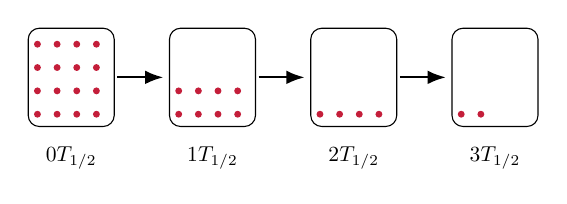
\begin{tikzpicture}[>=Latex,scale=.78,transform shape]\foreach \x/\n/\t in {0/16/0,2.3/8/1,4.6/4/2,6.9/2/3}{\draw[rounded corners] (\x,-.8) rectangle +(1.4,1.6);\foreach \i in {1,...,\n}{\pgfmathsetmacro{\xx}{\x+.15+mod(\i-1,4)*.32}\pgfmathsetmacro{\yy}{-.6+floor((\i-1)/4)*.38}\fill[ChinaRed] (\xx,\yy) circle (1.6pt);}\node[below] at (\x+.7,-1){\t $T_{1/2}$};}\draw[->,thick] (1.45,0)--(2.2,0);\draw[->,thick] (3.75,0)--(4.5,0);\draw[->,thick] (6.05,0)--(6.8,0);\end{tikzpicture}\end{columns}
\begin{exampleblock}{例題}3半減期後に残る割合は？\quad \ans{$(1/2)^3=1/8=12.5\%$。}\end{exampleblock}
\end{frame}

\begin{frame}{炭素14はどう生まれ、どう壊れるか}
\centering
\begin{tikzpicture}[>=Latex,node distance=10mm]
\node[draw,rounded corners,fill=SoftBlue,minimum width=34mm,minimum height=12mm] (n){宇宙線が作る中性子};
\node[draw,rounded corners,fill=SoftGreen,right=of n,minimum width=35mm,minimum height=12mm] (c){大気中の ${}^{14}$N};
\node[draw,rounded corners,fill=SoftRed,right=of c,minimum width=37mm,minimum height=12mm] (r){${}^{14}$C $+$ 陽子};
\draw[->,very thick] (n)--(c);\draw[->,very thick] (c)--node[above]{${}^{14}\mathrm{N}(n,p){}^{14}\mathrm{C}$}(r);
\end{tikzpicture}
\vspace{1em}
\begin{block}{$\beta^-$ 崩壊}\[{}^{14}_{6}\mathrm{C}\longrightarrow{}^{14}_{7}\mathrm{N}+e^-+\bar{\nu}_e\qquad T_{1/2}\approx5730\ \text{年}\]\end{block}
\begin{exampleblock}{例題}この崩壊で原子番号はどう変わるか。\quad \ans{6から7へ1増加。}\end{exampleblock}
\end{frame}

\begin{frame}{炭素14年代測定の考え方}
\begin{enumerate}\item 生物が生きている間：大气和食物からCを取り込み、${}^{14}$C比率近似一定。\item 死後：Cの取り込み停止。${}^{14}$Cだけが衰変。\item 残存率から死亡後の时间を估算。\end{enumerate}
\centering\begin{tikzpicture}[>=Latex]\draw[->](0,0)--(8,0)node[right]{時間};\draw[->](0,0)--(0,4.2)node[above]{残存率};\draw[JapanBlue,very thick] plot[smooth] coordinates{(0,4)(2,2)(4,1)(6,.5)(8,.25)};\foreach \x/\lab in {0/0,2/5730,4/11460,6/17190}{\draw (\x,.1)--(\x,-.1) node[below]{\lab};}\end{tikzpicture}
\end{frame}

\begin{frame}{炭素14：計算例題}
\def\exq{木片中の ${}^{14}$C の放射能が、現生木材の12.5\%だった。半減期を5730年とすると、木片の年代は約何年前か。}
\only<1>{\vfill\questioncard{\exq}\vfill}
\only<2>{\questioncard{\exq}\vfill\reasonflow{残存率12.5\%}{$(1/2)^3$}{3半減期}\vfill
\answercard{\centering\Large $t=3\times5730=\boxed{17190\ \text{年前}}$\qquad\small EJU基础题按理想半衰期模型。}}
\end{frame}

\section{まとめ}
\begin{frame}{総合チェック}
\small
\begin{enumerate}\item 空気、酸素、塩化ナトリウム水溶液を純物質／混合物に分類せよ。\item ヨウ素と砂を分ける方法を答えよ。\item 黒鉛が電気を通す理由を簡潔に述べよ。\item ${}^{14}_{6}$C の中性子数を答えよ。\item ${}^{14}$C が12.5\%残るまで何年か。\end{enumerate}
\begin{exampleblock}{解答}1 空気・塩化ナトリウム水溶液＝混合物；酸素＝純物質。\quad 2 昇華法。\quad 3 動ける電子がある。\quad 4 8。\quad 5 17190年。\end{exampleblock}
\end{frame}

\begin{frame}[shrink=8]{参考資料}
\small
\begin{block}{出題範囲・問題形式}日本学生支援機構（JASSO）「EJU 化学シラバス（2026年度第1回から）」\newline\url{https://www.jasso.go.jp/ryugaku/eju/examinee/syllabus/science_chem.html}\end{block}
\begin{block}{数値データ}NIST, \textit{CODATA Recommended Values of the Fundamental Physical Constants: 2022}.\newline\url{https://physics.nist.gov/cuu/Constants/}\end{block}
\begin{block}{炭素14}U.S. Geological Survey, \textit{Carbon-14 Dating}; IAEA, radiocarbon dating resources.\newline\url{https://pubs.usgs.gov/fs/1999/0190/report.pdf}\end{block}
\end{frame}
\end{document}
